%%%%%%%%%%%%%%
%% Run LaTeX on this file several times to get Table of Contents,
%% cross-references, and citations.

%% If you have font problems, you may edit the w-bookps.sty file
%% to customize the font names to match those on your system.

%% w-bksamp.tex. Current Version: Feb 16, 2012
%%%%%%%%%%%%%%%%%%%%%%%%%%%%%%%%%%%%%%%%%%%%%%%%%%%%%%%%%%%%%%%%
%
%  Sample file for
%  Wiley Book Style, Design No.: SD 001B, 7x10
%  Wiley Book Style, Design No.: SD 004B, 6x9
%
%
%  Prepared by Amy Hendrickson, TeXnology Inc.
%  http://www.texnology.com
%%%%%%%%%%%%%%%%%%%%%%%%%%%%%%%%%%%%%%%%%%%%%%%%%%%%%%%%%%%%%%%%

%%%%%%%%%%%%%
% 7x10
%\documentclass{wileySev}

% 6x9
\documentclass{wileySix}

\usepackage{graphicx}
\usepackage{listings}
\usepackage{float}
\usepackage[urlcolor=blue,colorlinks=true]{hyperref}
\usepackage{color}

\definecolor{codegreen}{rgb}{0,0.6,0}
\definecolor{codegray}{rgb}{0.5,0.5,0.5}
\definecolor{codepurple}{rgb}{0.58,0,0.82}
\definecolor{backcolour}{rgb}{0.95,0.95,0.92}

\lstdefinestyle{mystyle}{
    backgroundcolor=\color{backcolour},
    commentstyle=\color{codegreen},
    keywordstyle=\color{magenta},
    numberstyle=\tiny\color{codegray},
    stringstyle=\color{codepurple},
    basicstyle=\footnotesize,
    breakatwhitespace=false,
    breaklines=true,
    captionpos=b,
    keepspaces=true,
    numbers=left,
    numbersep=5pt,
    showspaces=false,
    showstringspaces=false,
    showtabs=false,
    tabsize=2,
    language=sh
}

\lstset{style=mystyle}

%%%%%%%
%% for times math: However, this package disables bold math (!)
%% \mathbf{x} will still work, but you will not have bold math
%% in section heads or chapter titles. If you don't use math
%% in those environments, mathptmx might be a good choice.

% \usepackage{mathptmx}

% For PostScript text
\usepackage{w-bookps}

%%%%%%%%%%%%%%%%%%%%%%%%%%%%%%%%%%%%%%%%%%%%%%%%%%%%%%%%%%%%%%%%
%% Other packages you might want to use:

% for chapter bibliography made with BibTeX
% \usepackage{chapterbib}

% for multiple indices
% \usepackage{multind}

% for answers to problems
% \usepackage{answers}

%%%%%%%%%%%%%%%%%%%%%%%%%%%%%%
%% Change options here if you want:
%%
%% How many levels of section head would you like numbered?
%% 0= no section numbers, 1= section, 2= subsection, 3= subsubsection
%%==>>
\setcounter{secnumdepth}{3}

%% How many levels of section head would you like to appear in the
%% Table of Contents?
%% 0= chapter titles, 1= section titles, 2= subsection titles,
%% 3= subsubsection titles.
%%==>>
\setcounter{tocdepth}{2}

%% Cropmarks? good for final page makeup
%% \docropmarks

%%%%%%%%%%%%%%%%%%%%%%%%%%%%%%
%
% DRAFT
%
% Uncomment to get double spacing between lines, current date and time
% printed at bottom of page.
% \draft
% (If you want to keep tables from becoming double spaced also uncomment
% this):
% \renewcommand{\arraystretch}{0.6}
%%%%%%%%%%%%%%%%%%%%%%%%%%%%%%

%%%%%%% Demo of section head containing sample macro:
%% To get a macro to expand correctly in a section head, with upper and
%% lower case math, put the definition and set the box
%% before \begin{document}, so that when it appears in the
%% table of contents it will also work:

\newcommand{\VT}[1]{\ensuremath{{V_{T#1}}}}

%% use a box to expand the macro before we put it into the section head:

\newbox\sectsavebox
\setbox\sectsavebox=\hbox{\boldmath\VT{xyz}}

%%%%%%%%%%%%%%%%% End Demo


\begin{document}


\booktitle{SIG (Sistem Informasi Geografis)}
\subtitle{Semester 5}

\authors{D4TI3B\\
\affil{Angkatan 2017}
%Floyd J. Fowler, Jr.\\
%\affil{University of New Mexico}
}

\offprintinfo{SIG (Sistem Informasi Geografis), First Edition}{D4TI3A}

%% Can use \\ if title, and edition are too wide, ie,
%% \offprintinfo{Survey Methodology,\\ Second Edition}{Robert M. Groves}

%%%%%%%%%%%%%%%%%%%%%%%%%%%%%%
%%
\halftitlepage

%\titlepage


\begin{copyrightpage}{2019}
%Survey Methodology / Robert M. Groves . . . [et al.].
%\       p. cm.---(Wiley series in survey methodology)
%\    ``Wiley-Interscience."
%\    Includes bibliographical references and index.
%\    ISBN 0-471-48348-6 (pbk.)
%\    1. Surveys---Methodology.  2. Social 
%\  sciences---Research---Statistical methods.  I. Groves, Robert M.  II. %
%Series.\\
%
%HA31.2.S873 2007
%001.4'33---dc22                                             2004044064
\end{copyrightpage}

\dedication{`Jika Kamu tidak dapat menahan lelahnya belajar,
Maka kamu harus sanggup menahan perihnya Kebodohan.'
~Imam Syafi'i~}

\begin{contributors}
\name{Rolly Maulana Awangga,} Informatics Research Center., Politeknik Pos Indonesia, Bandung,
Indonesia



\end{contributors}

\contentsinbrief
\tableofcontents
\listoffigures
\listoftables
\lstlistoflistings


\begin{foreword}
Sepatah kata dari Kaprodi, Kabag Kemahasiswaan dan Mahasiswa
\end{foreword}

\begin{preface}
Buku ini diciptakan bagi yang awam dengan flask sekalipun.

\prefaceauthor{R. M. Awangga}
\where{Bandung, Jawa Barat\\
Februari, 2019}
\end{preface}


\begin{acknowledgments}
Terima kasih atas semua masukan dari para mahasiswa agar bisa membuat buku ini 
lebih baik dan lebih mudah dimengerti.

Terima kasih ini juga ditujukan khusus untuk team IRC yang 
telah fokus untuk belajar dan memahami bagaimana buku ini mendampingi proses 
Intership.
\authorinitials{R. M. A.}
\end{acknowledgments}

\begin{acronyms}
\acro{ACGIH}{American Conference of Governmental Industrial Hygienists}
\acro{AEC}{Atomic Energy Commission}
\acro{OSHA}{Occupational Health and Safety Commission}
\acro{SAMA}{Scientific Apparatus Makers Association}
\end{acronyms}

\begin{glossary}
\term{git}Merupakan manajemen sumber kode yang dibuat oleh linus torvald.

\term{bash}Merupakan bahasa sistem operasi berbasiskan *NIX.

\term{linux}Sistem operasi berbasis sumber kode terbuka yang dibuat oleh Linus Torvald
\end{glossary}

\begin{symbols}
\term{A}Amplitude

\term{\hbox{\&}}Propositional logic symbol 

\term{a}Filter Coefficient

\bigskip

\term{\mathcal{B}}Number of Beats
\end{symbols}

\begin{introduction}

%% optional, but if you want to list author:

\introauthor{Rolly Maulana Awangga, S.T., M.T.}
{Informatics Research Center\\
Bandung, Jawa Barat, Indonesia}

Pada era disruptif  \index{disruptif}\index{disruptif!modern} 
saat ini. git merupakan sebuah kebutuhan dalam sebuah organisasi pengembangan perangkat lunak.
Buku ini diharapkan bisa menjadi penghantar para programmer, analis, IT Operation dan Project Manajer.
Dalam melakukan implementasi git pada diri dan organisasinya.

Rumusnya cuman sebagai contoh aja biar keren\cite{awangga2018sampeu}.

\begin{equation}
ABC {\cal DEF} \alpha\beta\Gamma\Delta\sum^{abc}_{def}
\end{equation}

\end{introduction}

%%%%%%%%%%%%%%%%%% Isi Buku %%%%%%%%%%%%%%%%%%
\chapter{Tugas Pertama}
\section{NAMA (NPM)}
\subsection{Pengertian}
\subsection{Sejarah}
\subsection{Koordinat}
\subsection{Data Geospasial}
\subsection{Link}
\subsection{Plagiarism}

\subsection{Cara Penggunaan}
\subsubsection{Gambar}

\hfill\break

Contoh Gambar
\begin{figure}[H]
	
\includegraphics[width=4cm]{figures/himatif.png}
	\centering
	\caption{Contoh gambar.}
\end{figure}

\subsubsection{List}
\begin{enumerate}
	\item Satu
	\item Dua
\end{enumerate}

\begin{itemize}
	\item Satu
	\item Dua
\end{itemize}


\section{Liyana Majdah Rahma(1174039)}
\subsection{Pengertian}

\subsection{Sejarah}
\subsection{Koordinat}
\subsection{Data Geospasial}
Data dalam Sistem Informasi Geografis terdiri dari dua komponen yaitu data spasial dan data attribute. Kata Geospasial terdiri dari dua katayaitu geo dengan spasial, Geo sendiri memiliki arti bumi sedangkan spasial memiliki arti ruang. Jika di gabungkan geospasial merupakan data bereferensi geografis atas resprentasi obyek dibumi. Selain itu juga geospasial  di bagi lagi menjadi dua bagian,yaitu data garis dengan data geometri. Data tersebut terdiri dari tiga elemen berupa,garis,titik,dan luasan. Serta Data geospasial berbentuk raster dan vector.

Model data vector merupakan data yang menampilkan,menempatkan,dan menyimpan data spasial dengan menggunaka titik dan garis,bahkan selain itu juga dapat berupa bentuk polygon. Biasanya jenis tipe data ini terdapat pada peta. Dalam format vector , bumi di representasikan sebagai suatu mosaic dari sebuah garis,polygon (dimana daerah yang dibatasi oleh garis yang berawal dan berakhir pada titik yang sama. Setiap Data pada vector dapat mempunyai informasi-informasi yang berasosiasi satu dengan yang lainnya misalnya penggunaan pada sebuah label untuk menggambarkan informasi pada suatu lokasi. Ada pun Keuntungan utama dari format data vektor yaitu adalah ketepatan dalam merepresentasikan fitur titik, batasan dan garis lurus. Hal tersebut juga  sangat berguna untuk analisa yang membutuhkan ketepatan posisi, misalnya pada basisdata batas-batas kadaster. Selain itu juga terdapat Kelemahan  saat menggunakan data vektor yang utama adalah ketidakmampuannya dalam mengakomodasi perubahan gradual.


Selanjutnya yang kedua model data raster merupakan data yang dihasilkan dari sistem Penginderaan Jauh. Pada data raster juga, obyek geografis direpresentasikan sebagai struktur sel grid yang disebut dengan pixel (picture element).  Selain itu  data raster, memiliki  resolusi (definisi visual) tergantung ukuran pixel-nya.  Resolusi  pixel juga dapat  menggambarkan ukuran sebenarnya di permukaan bumi yang diwakili oleh setiap pixel pada citra. Jika Semakin kecil ukuran permukaan bumi yang direpresentasikan oleh satu sel, maka semakin tinggi  hasil resolusinya. Begitupun data raster sangat baik untuk direpresentasikan pada batas-batas yang berubah secara gradual, misalnya pada  jenis tanah, kelembaban tanah, vegetasi, suhu tanah, dan lain-lainnya.


\subsection{Link}
\href{https://youtu.be/hFj3s-4dte8}{kli ini bro}
\subsection{Plagiarism}
\begin{figure}[H]
	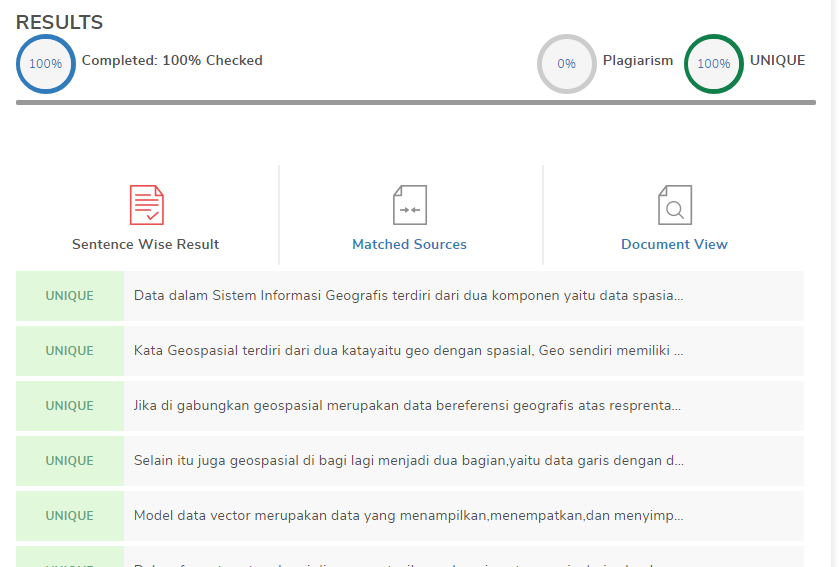
\includegraphics[width=4cm]{figures/1174039/plagiat.png}
	\centering
	\caption{Plagiat.}
\end{figure}


\section{FaisalNajibAbdullah(1174042)}

\subsection{Sejarah}
Sejarah geografi dimulai sejak manusia mulai berinteraksi dengan lingkunganya, hal ini juga merupakan awal mula dari berkembangnya ilmu pengetahuan tentang geografi.
Pada awal dikenalnya sistem informasi geografis bahwa tidak lepas dari adanya kemajuan didalam bidang teknologi. Pada awal tahun 1960 perkembangan sistem informasi geografis dalam ilmu komputer semakin pesat dan siap dingunakan pada bidang milliter. Pada taun 1700 teknik yang digunakan pada survei modern untuk pemetaan topografis digunakan atau diterapkan , hal ini juga termasuk pada versi awal pemetaan tematis.
Pada 35000 tahun yang lalu, di sebuah dinding tepatnya di gua Lascaux, Perancis, para pemburu Cro-Magnon menggambarkan hewan-hewan mangsa mereka. Mereka juga menggambarkan garis-garis yang dipercaya sebagai rute dari migrasi hewan-hewan mangsa mereka tersebut. Catatan awal tersebut sejalan dengan dua elemen struktur pada sistem informasi geografis modern saat ini, arsip grafis yang terhubung ke database atribut. 
Lalu pada tahun 1700-an teknik survei modern untuk pemetaan topografis diterapkan, termasuk versi awal pemetaan tematis, contohnya untuk keilmuan atau data sensus. 
\begin{figure}[H]
	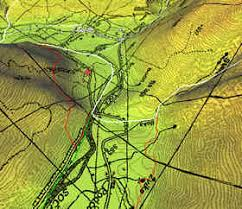
\includegraphics[width=4cm]{figures/1174042/gis.jpg}
	\centering
	\caption{Sejarah Gis}
\end{figure}

\subsection{Link}
\href{https://www.youtube.com/watch?v=8gTLBneTUAo&t=15s}{Youtube}
\subsection{Plagiarism}
\begin{figure}[H]
	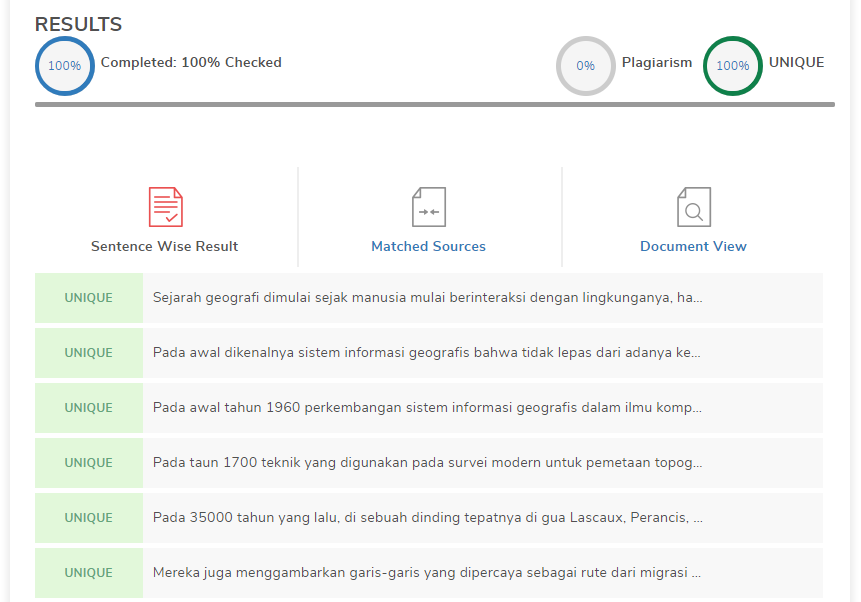
\includegraphics[width=4cm]{figures/1174042/plagiat.png}
	\centering
	\caption{Plagiarism}
\end{figure}
\section{Alit fajar Kurniawan (1174057)}

\subsection{Pengertian}
Geografi adalah ilmu pengetahuan yang mengambarkan segala sesuatu yang ada di permukaan bumi. \hfill\break
Geografi juga selain mempelajari bagian permukaan bumi, tapi juga mempelajari seluruh bagian bumi mulai darti struktur bumi,jenis batuan yang menyusun bumi serta atmosfer yang melindungi bumi. \hfill\break
Segala aktifitas yang terjadi di bumi merupakan bagian dari ilmu Geografi.\hfill\break
\subsection{Sejarah}
Sejarah geografi dimulai sejak manusia mulai berinteraksi dengan lingkunganya, hal ini juga merupakan awal mula dari berkembangnya ilmu pengetahuan tentang geografi.\hfill\break
Pada awalnya geografi hanya membahas atau mendekripsikan gambaran umum tentang fakta-fakta yang menjelaskan keadaan di muka bumi. Pada abad ke-18 yaitu masa geografi klasik, ilmu geografi hanya sebatas menjelaskan dan mengumpulkan informasi tentang lingkungan geografi saja, misalnya: keadaan politik, industri, iklim terutama di kota-kota besar.\hfill\break
Sejarah geografi terus berjalan dan berkembang. Tepatnya, diabad ke-19 geografi mengalami perkembangan dari segi keilmuannya. Dari yang semula hanya mendeskripsikan saja kemudian berkembang menjadi lebih spesifik yaitu dengan menjelaskan lingkungan geografi secara sistematis.\hfill\break
Pada pertengahan abad ke-19, keilmuan dalam geografi sudah membahas sampai ketingkat membandingkan keadaan, data geografis dan karakteristik antara wilayah yang satu dengan wilayah yang lain di muka bumi. Hal ini kita kenal sebagai “Comparative Geography”.\hfill\break
Perkembangan keilmuwan geografi semakin pesat pasca terjadinya perang dunia ke-II. Yang semula dikembangkan oleh imuwan Amerika dan Inggris yang dikenal sebagai “Comparative Geography” kemudian berkembang menjadi “Global Geography” dimana objek kajiannya semakin luas yaitu meliputi seluruh dunia. Era inilah yang dinamakan sebagai “era geografi modern”.\hfill\break
Dari pembahasan di atas, kita sudah mengetahui kapan sejarah geografi itu dimulai yaitu sejak adanya interaksi antara manusia dengan lingkungannya. Bila seperti itu, maka hakekatnya sejak Nabi Adam as turun ke bumi sebetulnya geografi sudah ada.\hfill\break
Akan tetapi penggalian geografi secara keilmuan sendiri baru dilakukan pertama kali oleh orang-orang Yunani. Dimana pada perkembangan awalnya dilatarbelakangi oleh suatu upaya masyarakat Yunani untuk melepaskan diri dari alam pikiran dan kepercayaan. Dimana kepercayaan tersebut meyakini bahwa dewa-dewa ikut turut campur dalam segala bentuk kejadian di bumi.\hfill\break
Istilah geografi sebenarnya baru digunakan pada tahun 1972 sedangkan sebelumnya lebih menggunakan istilah “ilmu bumi”. Istilah ini pertama kali diperkenalkan oleh seorang ahli filsafat dan astronomi yang bernama Eratosthenes pada 276 194 sebelum masehi.Kemudian, Claudius Ptoleumaeus melakukan peletakan dasar-dasar keilmuan geografi.\hfill\break
Sejarah perkembangan geografi terus berlanjut. Immanuel Kant mengembangkan geografi modern kemudian Karl Ritter juga mengembangkan geografi sosial.\hfill\break
Selain itu ada tokoh-tokoh lain yang ikut andil dalam mengembangkan geografi yaitu Alexander von Humbolt sebagai peletak dasar geografi fisika modern dan sebagainya.\hfill\break

\begin{figure}[H]
	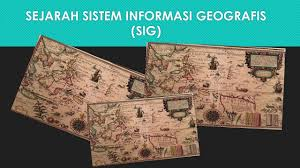
\includegraphics[width=4cm]{figures/1174057/sejarah.jpg}
	\centering
	\caption{Sejarah Gis}
\end{figure}

\subsection{Link}
\href{https://www.youtube.com/watch?v=XdUSIKaI3zc}{Nonton Video aku di Youtube}
\subsection{Plagiarism}
\begin{figure}[H]
	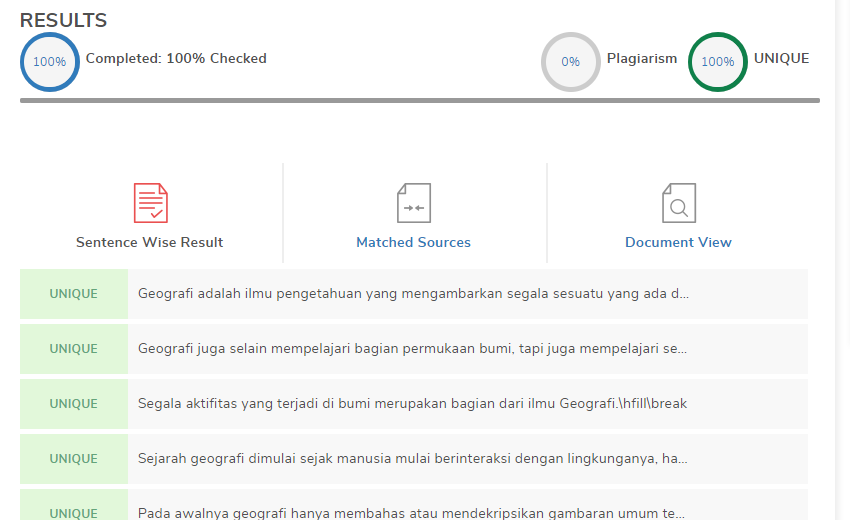
\includegraphics[width=4cm]{figures/1174057/plagiarisme.png}
	\centering
	\caption{Plagiarism}
\end{figure}
\section{Luthfi Muhammad Nabil (1174035)}
\subsection{Data Geospasial}
Data Geospasial merupakan data yang isinya mengenai lokasi geografis, ukuran atau karakteristik obyek alam atau buatan manusia yang berada di lingkungan bumi baik di bawah permukaan, permukaan, atau atas permukaan. Objek yang dimaksud pada data geospasial salah satunya mencakup jalan, bangunan, gunung, laut, dan sebagainya. Untuk bentuk data geospasial sendiri berbentuk data vektor dan data gambar yang dibuat menjadi kumpulan data untuk aplikasi dapat memproses data tersebut. Selain data tersebut, informasi mengenai karakteristik obyek juga disimpan pada data geospasial seperti nama jalan, ukuran bangunan, nama tempat, dan lain sebagainya.
\break
Data Geospasial bersumber dari beberapa hal berikut : 
\begin{itemize}
	\item Rekaman Data Alat Permukaan : Untuk merekam data yang realtime, alat akan berperan pada pengiriman data geospasial. Alat yang dimaksud sepert Sensor pada Arduino.
	\item Satelit Luar Angkasa : Selain permukaan, data secara keseluruhan juga diperlukan untuk membuat data keseluruhan permukaan bumi dan data lainnya. 
	\item Data Pemerintah : Data yang sudah diukur oleh pemerintah sebelumnya juga akan dipakai untuk membuat karakteristik detail dari sebuah obyek. 
	\item Dan lain sebagainya.
\end{itemize}
Data geospasial sudah banyak digunakan pada banyak aplikasi. Data yang akan dipakai untuk menunjukan lokasi, tata letak daerah, dan sebagainya. Data geospasial juga memberi manfaat bagi yang menggunakan atau yang merasakan aplikasi yang memakai Data geospasial. Beberapa manfaat yang bisa didapat diantaranya : 
\begin{itemize}
	\item Dapat mencari sebuah tujuan hanya dengan menuliskan nama tempat atau alamat
	\item Mengetahui kondisi dari daerah berdasarkan data geospasial realtime yang dibuat oleh setempat
	\item Sebagai survey untuk beberapa lokasi yang perlu diperhatikan
	\item Sebagai pembelajaran mengenai geografis
\end{itemize}
\subsection{Link}
\subsection{Plagiarism}
\begin{figure}[H]
	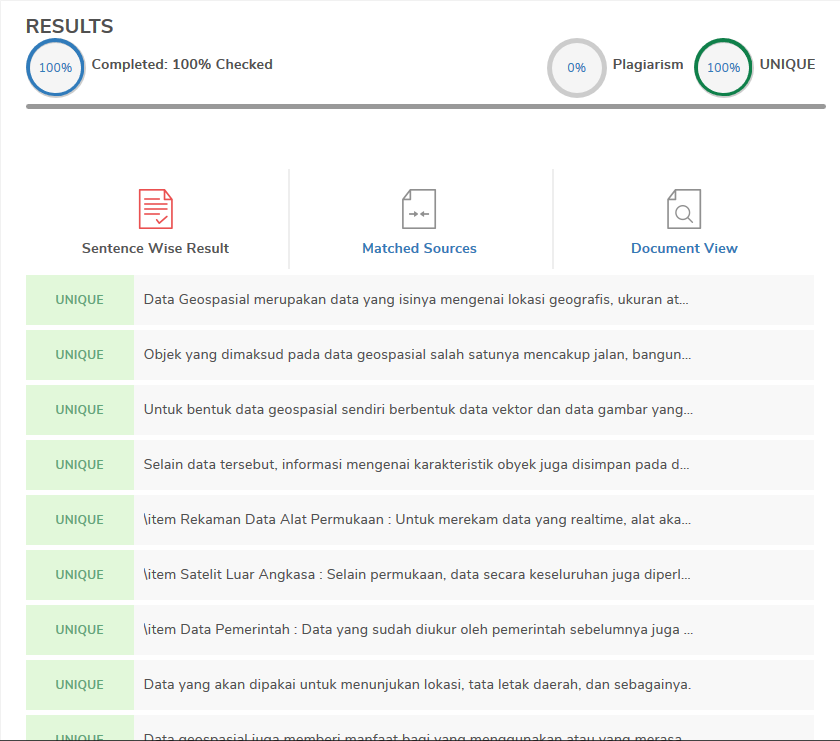
\includegraphics[width=10cm]{figures/1174035/tugas1/plagiat.png}
	\centering
	\caption{Hasil Pengecekan Plagiat}
\end{figure}


\section{Hagan Rowlenstino A. S (1174040)}
\subsection{Pengertian}
Sistem Informasi Geografis adalah sebuah sistem informasi yang berbasis computer yang dirancang sedemikian rupa untuk bekerja dengan menggunakan data yang memiliki informasi spasial yang bereferensikan keuangan. Sistem ini akan menangkap(capture), mengecek, mengintegrasikan, memanipulasi, menganalisa serta menampilkan data yang secara spasial mereferensikan kondisi bumi.
Menurut ahli :
\begin{enumerate}
	\item Marbel et al (1983), GIS adalah sistem penanganan keruangan
	\item Berry (1988), GIS adalah sistem informasi, referensi internal, serta otomatisasi data keruangan.
\end{enumerate}

4 SUBSISTEM GIS :
\begin{enumerate}
	\item Data Input : mengumpulkan, mempersiapkan, dan menyimpan data spasial dan atributnya dari berbagai sumber
	\item Data output : menampilkan keluaran data dari sistem dalam bentuk tabel, grafik, peta , atau laporan
	\item Data Management : Mengorganisasikan data.
	\item Data Manipulation dan analysis : manipulasi dan permodelan data untuk menghasilkan informasi yang dihasilkan oleh GIS.
\end{enumerate}
Tugas Utama SIG :
\begin{enumerate}
	\item Konversi data dari peta kertas atau foto ke dalalm bentuk digital (digitalizing).
	\item Membuat peta digital.
	\item Memanipulasi atau transformasi agar data – data tersebut kompatibel dengan sistem
	\item Analisis query untuk melihat pola dan trend
	\item Memvisualisasikan hasil dengan peta atau graf
\end{enumerate}
Contoh di beberapa bidang :
\begin{itemize}
	\item SDA : studi kelayakan untuk tanaman pertanian, pengelolaan hutan, dll.
	\item Transportasi : analisis rawan macet dan kecelakaan
	\item Militer : penyediaan data spasial untuk rute perjalanan logistic, peralatan perang, dll.
\end{itemize}

\subsection{Link}
\href{https://www.youtube.com/watch?v=oCACYiDI29s}{Youtube Hagan}
\subsection{Plagiarism}

\begin{figure}[H]
	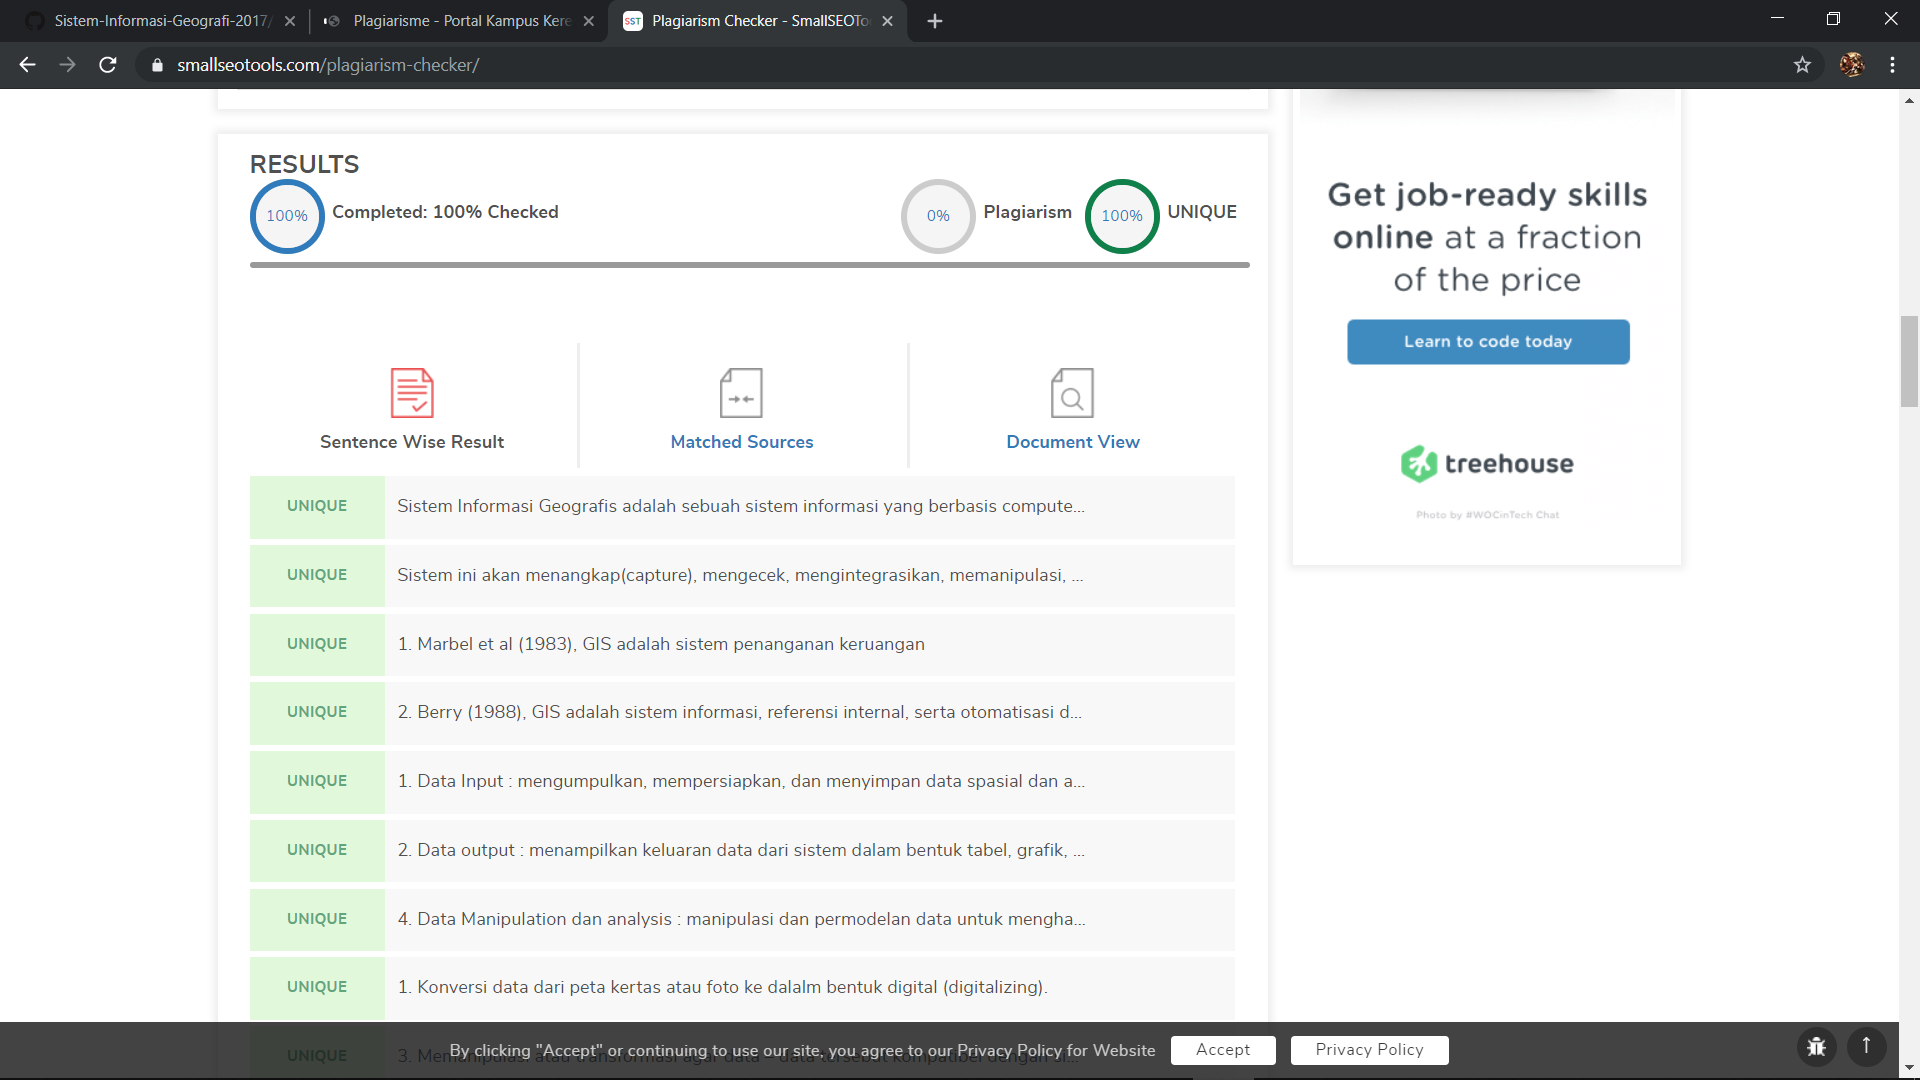
\includegraphics[width=4cm]{figures/1174040/1174040_plagiat_1.png}
	\centering
	\caption{Plagiarisme Hagan}
\end{figure}



\section{IrvanRizkiasyah - 1174043}
	\subsection{Data Geospasial}
	Istilah data geospasial dapat juga diganti dengan data spasial atau data GIS (geospatial information system data) yang merupakan sebuah data mengenai aspek fisik dan administratif dari sebuah objek geografis. Aspek fisik di sini mencakup pula bentuk anthropogenic dan bentuk alam baik yang terdapat di permukaan maupun di bawah permukaan bumi. Bentuk anthropogenic mengandung di dalamnya fenomena budaya seperti jalan, rel kereta api, bangunan, jembatan, dan sebagainya. Bentuk alam tentu saja adalah sungai, danau, pantai, daratan tinggi, dan sebagainya. Sedangkan aspek administratif adalah pembagian atau pembatasan sosio-kultural yang dibuat oleh suatu organisasi atau badan untuk keperluan pengaturan dan pemakaian sumberdaya alam.
	
	Sumber dari data geospasial dapat berupa :
	\begin{itemize}
		\item Data sistem penentuan posisi global (GPS). Data GPS dikumpulkan melalui sistem navigasi radio berbasis satelit dan darat. Smartphone berkemampuan GPS dapat memberikan lokasi seseorang.
		\item Data penginderaan jauh, melibatkan sebuah instrumen khusus yang digunakan untuk menangkap data yang bisa diubah menjadi dalam bentuk digital. Pemindai, satelit dan sistem radar merupakan contoh dari instrumen ini. Salah satu contoh dari penginderaan jauh ini adalah foto udara.
	\end{itemize}
	
	Foto udara dapat digunakan untuk mengenali beberapa obyek yang ada di muka bumi. Dengan menganalisa bentuk, ukuran dan warna obyek ini, kita dapat mengamati adanya tanah basah atau kering, tanaman sehat atau tanaman terserang penyakit, serta sawah irigasi atau sawah tadah hujan. Tanah basah akan berwarna lebih gelap bila dibandingkan dengan tanah yang kering.

	\subsection{Link video Data Geospasial}
		\href{https://youtu.be/w1NwuEcDHfA} {Link video Data Geospasial Irvan Rizkiansyah - 1174043}
		
	\subsection{Plagiarism}
	\begin{figure}[H]
		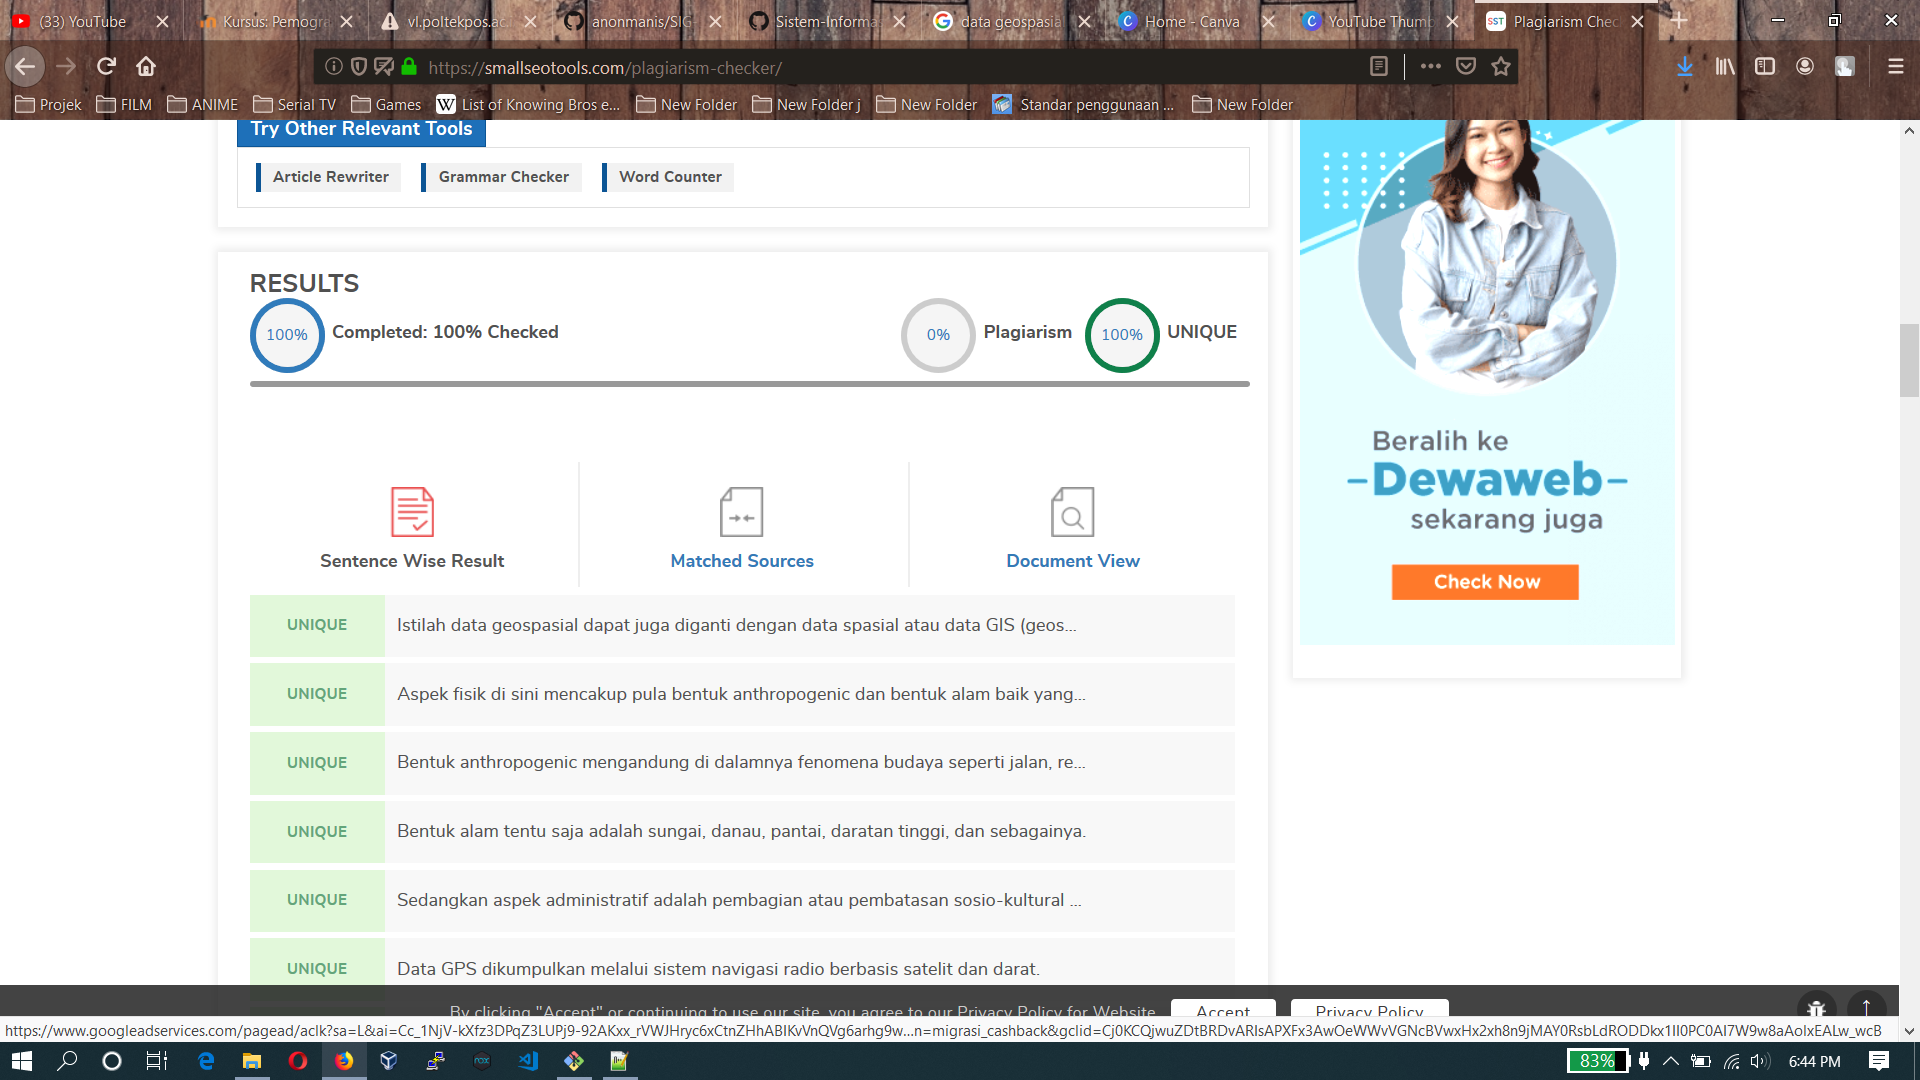
\includegraphics[width=10cm]{figures/1174035/Plagiarisme.png}
		\centering
		\caption{Hasil Pengecekan Plagiarisme}
	\end{figure}
\section{Dika Sukma Pradana(1174050)}

\subsection{Koordinat}
\par
Koordinat adalah sistem koordinat yang memungkinkan setiap lokasi di Bumi ditentukan oleh serangkaian angka, huruf, atau simbol. Koordinat sering dipilih sedemikian sehingga salah satu angka mewakili posisi vertikal dan dua atau tiga angka mewakili posisi horisontal; sebagai alternatif, posisi geografis dapat diekspresikan dalam vektor Kartesius tiga dimensi. Pilihan umum koordinat adalah lintang, bujur dan ketinggian. Untuk menentukan lokasi di pesawat membutuhkan proyeksi peta. secara singkanya yaitu salah satu dari dua garis lintang dan bujur yang persimpangannya menentukan titik geografis suatu tempat.


\begin{figure}[H]
	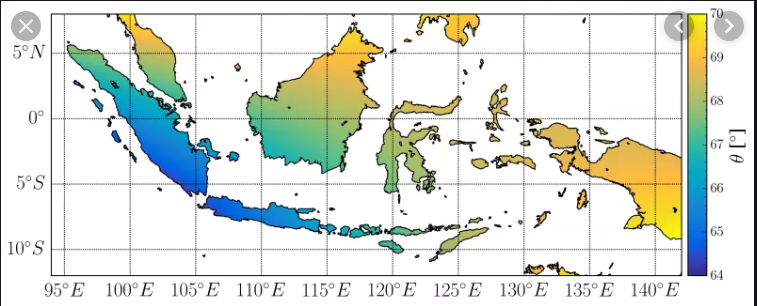
\includegraphics[width=4cm]{figures/1174050/koordinat.png}
	\centering
	\caption{Koordinat Indonesia}
\end{figure}

\subsection{Link}
\href{https://www.youtube.com/watch?v=GnI25H4HATo}{LINK Youtub, JANGAN LUPA SASKREB}
\subsection{Plagiarism}
\begin{figure}[H]
	\includegraphics[width=4cm]{figures/1174050/plagiarism.png}
	\centering
	\caption{Plagiarism}
\end{figure}
\section{MuhammadIqbalPanggabean(1174063)}

\subsection{Koordinat}
Koordinat didapatkan dari hasil perpotongan antara garis latitude (Y) / lintang dan garis longitude(X) / garis bujur sehingga bisa menunjukan suatu lokasi pada suatu daerah. \hfill\break 
Umumnya koordinat dibedakan menajadi koordinat Geografi dan Universal Transver Mercator(UTM). Pada koordinat geografi dibedakan menajadi 3 yaitu : \hfill\break
\begin{itemize}
	\item Degree, Decimal(DD, DDDD) contoh S 4.56734 E 102.67235
	\item Degree,Minute(DD MM,MMMM) contoh S 4 42,5423’ E 105 34,6445’
	\item Degree, Minute, Second(DD MM SS,SS) contoh : S 4 43’ 45,22 E 103 33’ 33,25
\end{itemize}
\hfill\break
\begin{figure}[H]
	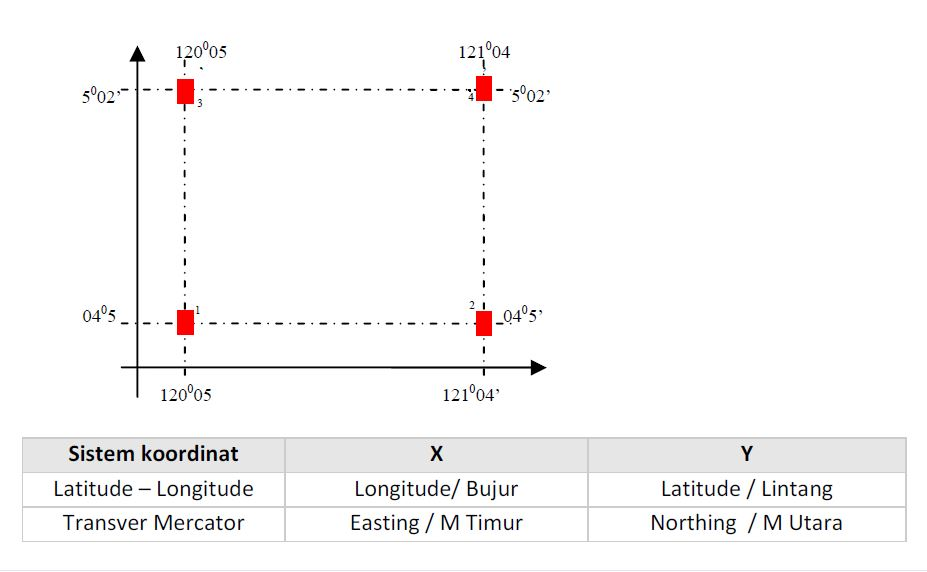
\includegraphics[width=4cm]{figures/1174063/koordinat.jpg}
	\centering
	\caption{Contoh Koordinat}
\end{figure}
Pada system koordinat UTM biasanya terdapat pembagian waktu berdasarkan zonasinya. \hfill\break
\begin{figure}[H]
	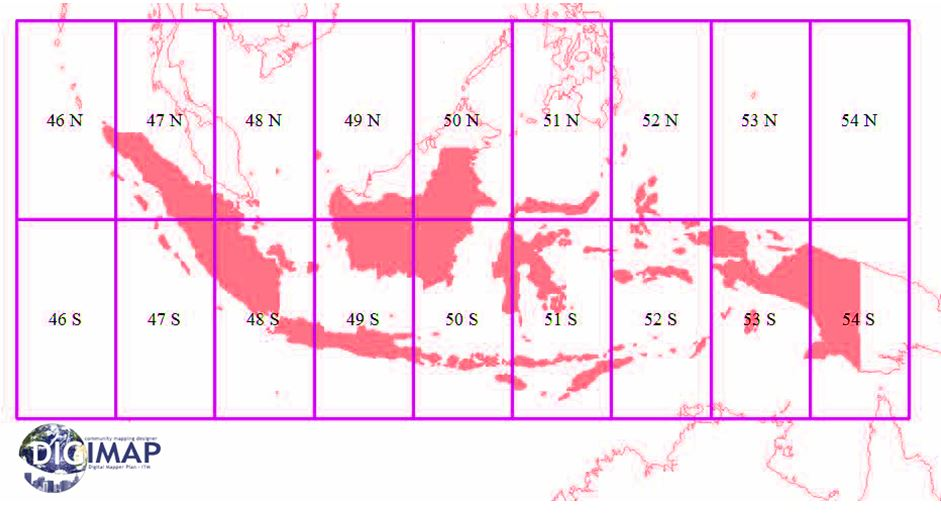
\includegraphics[width=4cm]{figures/1174063/utm.jpg}
	\centering
	\caption{Contoh Koordinat UTM}
\end{figure}

	\subsection{Link}
\href{https://youtu.be/mU4dPSOHDWI}{LOOK AT THIS}
\subsection{Plagiarism}
\begin{figure}[H]
	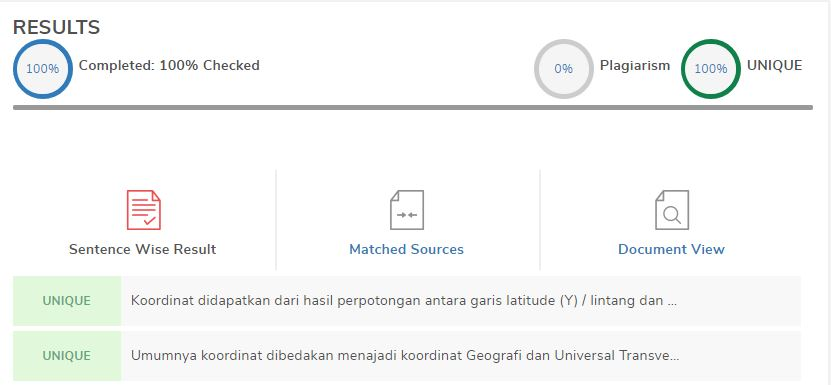
\includegraphics[width=4cm]{figures/1174063/plagiat.jpg}
	\centering
	\caption{Plagiat.}
\end{figure}


\section{Kevin Natanel Nainggolan(1174059)}
\subsection{Data Geospasial}
Apa itu DATA GEOSPASIAL, dua kata yang berasal dari geo dan spasial, dimana arti daripada geo sendiri adalah bumi dan spasial berarti raung. Data Geospasial dipecah menjadi dua jenis data, yaitu : 
\begin {enumerate}
	\item Data Grafis, terdiri dari tiga elemen, diantaranya:
		\begin {itemize}
			\item Titik
			\item Garis
			\item Luasan
		\end {itemize}
	\item Data Atribut
\end {enumerate}

\subsubsection{Tipe Data Vektor}
Data Vektor digunakan pada Geospasil pada titik koordinat yang menampilkan, menempatkan, dan menyimpan data spacial dengan elemen data grafis atau geometri, seperti yang sudah dibahas diatas, terdapat beberapa jenis tipe data vektor, diantaranya: 
\begin {itemize}
	\item Titik
	\item Garis
	\item Polygon
\end {itemize}
Tipe data yang sudah dituliskan di atas biasanya terletak pada peta, dan setiap bagian dari data tersebut bisa mempunyai informasi yang berhubungan satu dengan yang lainnya

\subsubsection{Tipe Data Line}
Data Line atau garis berbentuk satu dimensi yang menghubungkan dua titik atau lebih, biasanya Data Line digunakan untuk menunjukan objek geometri linear. Hal ini yang akan bergantung pada peta karena menjadi sumber atau skala representasi sebagai objek dengan menampilkan bentuk geometri garis.

\subsubsection{Raster}
Data grid atau raster mewakili tipe fitur permukaan, data ini berbasis sel dengan kategori data yang mencangkup citra udara dan satelit. Berikut jenis data raster:
\begin {itemize}
	\item Kontinu
	\item Diskrit
\end {itemize}

 
\subsection{Link}
\href{https://www.youtube.com/watch?v=gFEpzbs1_04}{Klik disini Untuk video dari geospasial selengkapnya}
\subsection{Plagiarism}
\begin{figure}[H]
	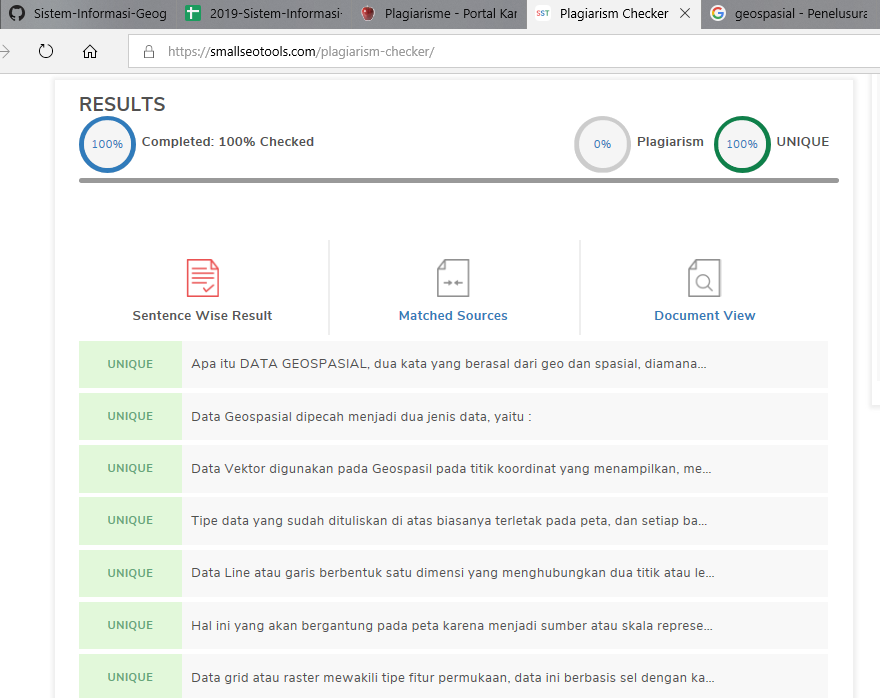
\includegraphics[width=4cm]{figures/1174059/plagiarisme.png}
	\centering
	\caption{Check Plagiat Kevin}
\end{figure}


\section{Teddy Gideon Manik(1174038)}

\subsection{Koordinat}
\par
Koordinat adalah sistem koordinat yang memungkinkan setiap lokasi di Bumi ditentukan oleh serangkaian angka, huruf, atau simbol. Koordinat sering dipilih sedemikian sehingga salah satu angka mewakili posisi vertikal dan dua atau tiga angka mewakili posisi horisontal; sebagai alternatif, posisi geografis dapat diekspresikan dalam vektor Kartesius tiga dimensi. Pilihan umum koordinat adalah lintang, bujur dan ketinggian. Untuk menentukan lokasi di pesawat membutuhkan proyeksi peta. secara singkanya yaitu salah satu dari dua garis lintang dan bujur yang persimpangannya menentukan titik geografis suatu tempat.
Dalam geometri, sistem koordinat adalah suatu sistem yang menggunakan satu atau lebih bilangan, atau koordinat, untuk secara unik menentukan posisi suatu titik atau unsur geometris lain pada manifold seperti ruang Euklides. Urutan koordinat adalah signifikan, dan mereka kadang-kadang diidentifikasi oleh posisi mereka dalam tuple dan kadang-kadang dengan huruf, seperti dalam "x-coordinate". Koordinat diambil untuk menjadi bilangan real dalam matematika dasar, tetapi mungkin bilangan kompleks atau elemen-elemen dari sistem yang lebih abstrak seperti sebuah cincin komutatif. Penggunaan sistem koordinat memungkinkan masalah dalam geometri untuk diterjemahkan ke dalam masalah-masalah tentang angka dan sebaliknya; ini adalah dasar dari geometri analitis.[3]


\begin{figure}[H]
	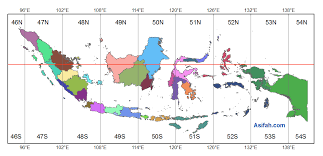
\includegraphics[width=4cm]{figures/1174038/peta koordinat indonesia.png}
	\centering
	\caption{Koordinat Indonesia}
\end{figure}

\subsection{Link}
\href{https://https://youtu.be/gIAfrXKGDCI}{LINK Youtub, JANGAN LUPA SASKREB}
\subsection{Plagiarism}
\begin{figure}[H]
	\includegraphics[width=4cm]{figures/1174038/plagiarism.png}
	\centering
	\caption{Plagiarism}
\end{figure}
\section{Ichsan Hizman Hardy(1174034)}

\subsection{Koordinat}
\par
Koordinat adalah sistem koordinat yang memungkinkan setiap lokasi di Bumi ditentukan oleh serangkaian angka, huruf, atau simbol. Koordinat sering dipilih sedemikian sehingga salah satu angka mewakili posisi vertikal dan dua atau tiga angka mewakili posisi horisontal; sebagai alternatif, posisi geografis dapat diekspresikan dalam vektor Kartesius tiga dimensi. Pilihan umum koordinat adalah lintang, bujur dan ketinggian. Untuk menentukan lokasi di pesawat membutuhkan proyeksi peta. secara singkanya yaitu salah satu dari dua garis lintang dan bujur yang persimpangannya menentukan titik geografis suatu tempat.


\begin{figure}[H]
	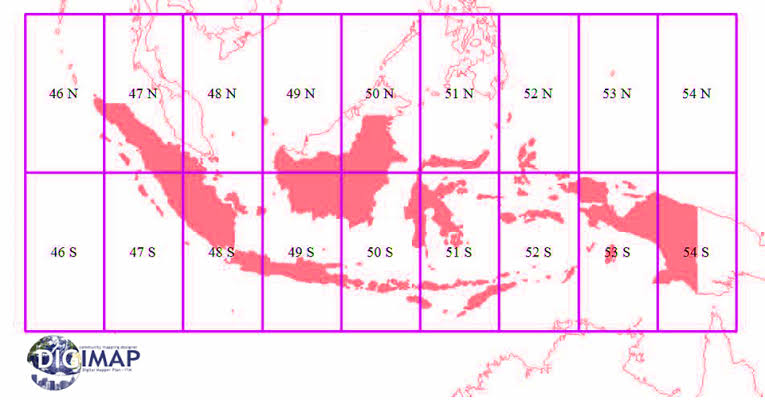
\includegraphics[width=4cm]{figures/1174034/koordinat.png}
	\centering
	\caption{Koordinat Indonesia}
\end{figure}

\subsection{Link}
\href{https://youtu.be/SxklV9IEFhc}{LINK Youtub, JANGAN LUPA SASKREB}
\subsection{Plagiarism}
\begin{figure}[H]
	\includegraphics[width=4cm]{figures/1174034/plagiarism.png}
	\centering
	\caption{Plagiarism}
\end{figure}


\chapter{Tugas Kedua}
\section{Liyana Majdah Rahma(1174039)}
\subsection{Point Polyline dan Polygon}
\begin{enumerate}
	\item 
	\lstinputlisting{src/1/1174039/soal1.py}
	\begin{figure}[H]
		
\includegraphics[width=12cm]{figures/1174042/No1.JPG}
		\centering
		\caption{Point}
	\end{figure}
	
	\item 
	\lstinputlisting{src/1/1174042/No2.py}
	\begin{figure}[H]
		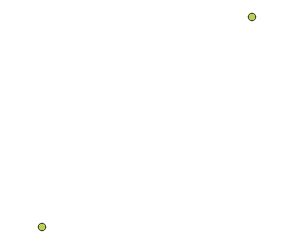
\includegraphics[width=12cm]{figures/1174042/No2.JPG}
		\centering
		\caption{Point}
	\end{figure}
	
	\item 
	\lstinputlisting{src/1/1174042/No3.py}
	\begin{figure}[H]
		
\includegraphics[width=12cm]{figures/1174042/No3.JPG}
		\centering
		\caption{Point}
	\end{figure}
	
	\item 
	\lstinputlisting{src/1/1174042/No4.py}
	\begin{figure}[H]
		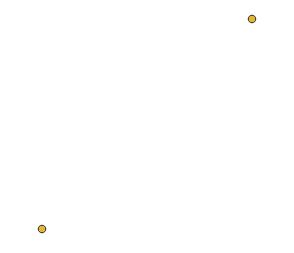
\includegraphics[width=12cm]{figures/1174042/No4.JPG}
		\centering
		\caption{Point}
	\end{figure}
	
	\item 
	\lstinputlisting{src/1/1174042/No5.py}
	\begin{figure}[H]
		
\includegraphics[width=12cm]{figures/1174042/No5.JPG}
		\centering
		\caption{Polyline}
	\end{figure}
	
	\item 
	\lstinputlisting{src/1/1174042/No6.py}
	\begin{figure}[H]
		
\includegraphics[width=12cm]{figures/1174042/No6.JPG}
		\centering
		\caption{Poligon}
	\end{figure}
	
	\item 
	\lstinputlisting{src/1/1174042/No7.py}
	\begin{figure}[H]
		
\includegraphics[width=12cm]{figures/1174042/No7.JPG}
		\centering
		\caption{Polygon}
	\end{figure}
	
	\item 
	\lstinputlisting{src/1/1174042/No8.py}
	\begin{figure}[H]
		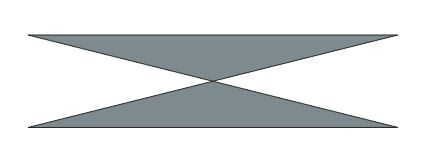
\includegraphics[width=12cm]{figures/1174042/No8.JPG}
		\centering
		\caption{Polygon}
	\end{figure}
	
	\item 
	\lstinputlisting{src/1/1174042/No9.py}
	\begin{figure}[H]
		
\includegraphics[width=12cm]{figures/1174042/No9.JPG}
		\centering
		\caption{Polygon}
	\end{figure}
	
	\item 
	\lstinputlisting{src/1/1174042/No10.py}
	\begin{figure}[H]
		
\includegraphics[width=12cm]{figures/1174042/No10.JPG}
		\centering
		\caption{Hasil mod saya yaitu 2 jadi yang saya kerjakan Bujursangkan yang berjum lah 4, Polygon}
	\end{figure}	
\end{enumerate}

\subsection{Link}
\href{https://youtu.be/4O3oxQESyjM}{Youtube}
\section{Liyana Majdah Rahma(1174039)}
\subsection{Point Polyline dan Polygon}
\begin{enumerate}
	\item 
	\lstinputlisting{src/1/1174039/soal1.py}
	\begin{figure}[H]
		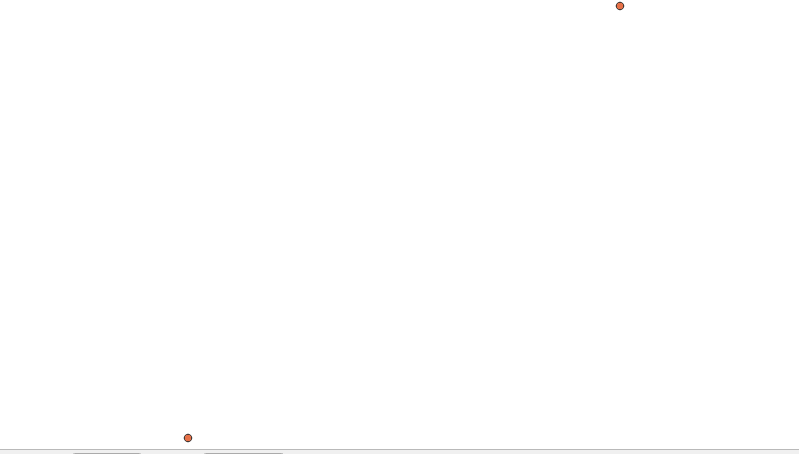
\includegraphics[width=12cm]{figures/1174039/gambar/hasil1.PNG}
		\centering
		\caption{Point}
	\end{figure}
	
	\item 
	\lstinputlisting{src/1/1174039/soal2.py}
	\begin{figure}[H]
		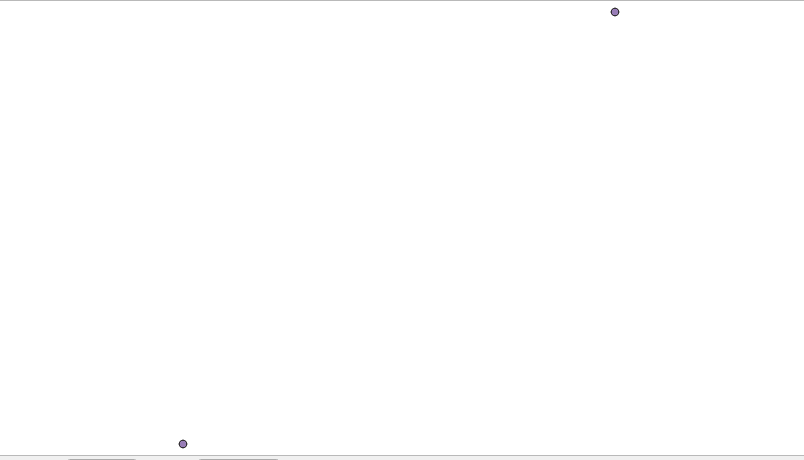
\includegraphics[width=12cm]{figures/1174039/gambar/hasil2.PNG}
		\centering
		\caption{Point}
	\end{figure}
	
	\item 
	\lstinputlisting{src/1/1174039/soal3.py}
	\begin{figure}[H]
		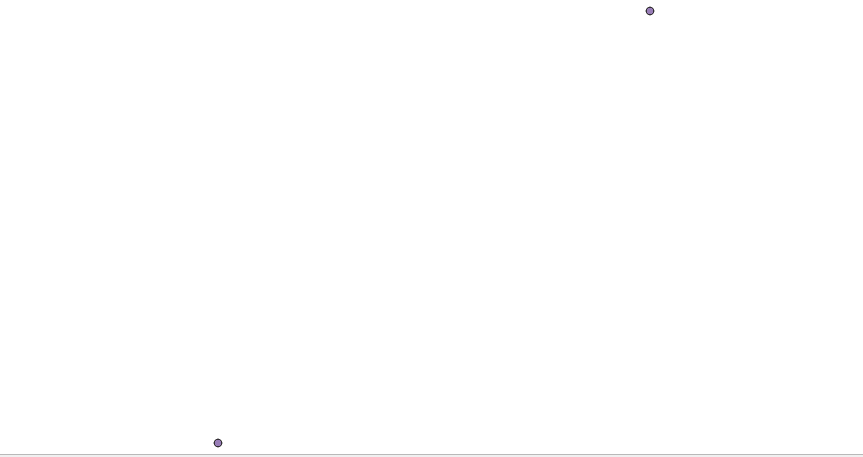
\includegraphics[width=12cm]{figures/1174039/gambar/hasil3.PNG}
		\centering
		\caption{Point}
	\end{figure}
	
	\item 
	\lstinputlisting{src/1/1174039/soal4.py}
	\begin{figure}[H]
		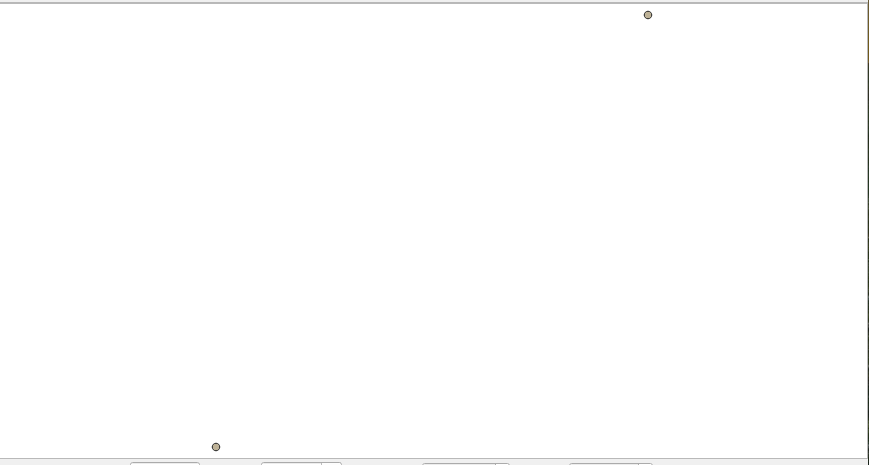
\includegraphics[width=12cm]{figures/1174039/gambar/hasil4.PNG}
		\centering
		\caption{Point}
	\end{figure}
	
	\item 
	\lstinputlisting{src/1/1174039/soal5.py}
	\begin{figure}[H]
		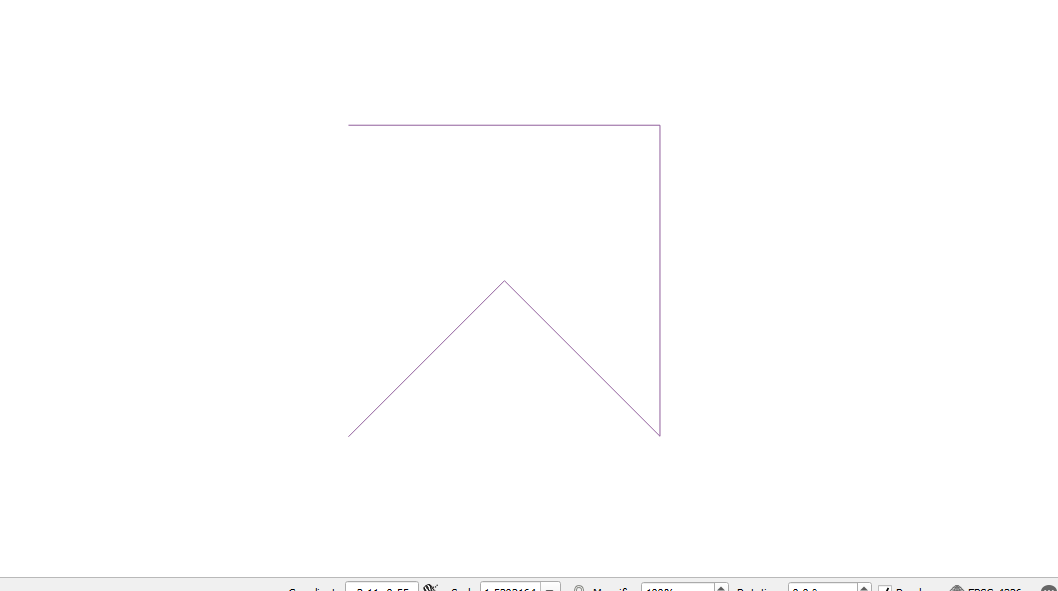
\includegraphics[width=12cm]{figures/1174039/gambar/hasil5.PNG}
		\centering
		\caption{Polyline}
	\end{figure}
	
	\item 
	\lstinputlisting{src/1/1174039/soal6.py}
	\begin{figure}[H]
		
\includegraphics[width=12cm]{figures/1174039/gambar/hasil6.PNG}
		\centering
		\caption{Poligon}
	\end{figure}
	
	\item 
	\lstinputlisting{src/1/1174039/soal7.py}
	\begin{figure}[H]
		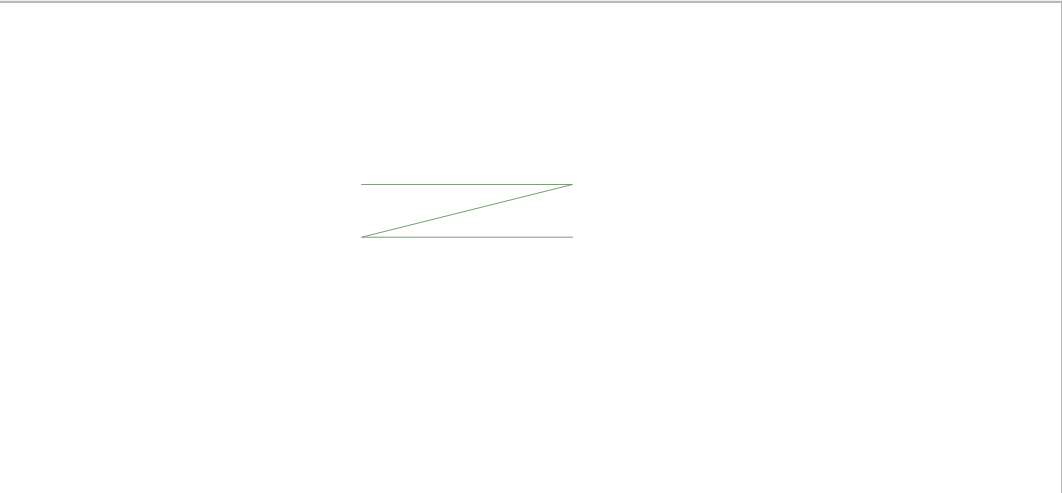
\includegraphics[width=12cm]{figures/1174039/gambar/hasil7.PNG}
		\centering
		\caption{Polygon}
	\end{figure}
	
	\item 
	\lstinputlisting{src/1/1174039/soal8.py}
	\begin{figure}[H]
		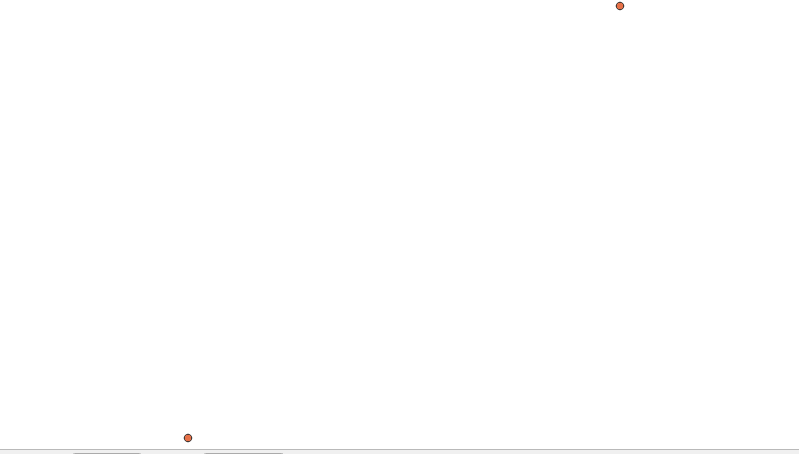
\includegraphics[width=12cm]{figures/1174039/gambar/hasil1.PNG}
		\centering
		\caption{Polygon}
	\end{figure}
	
	\item 
	\lstinputlisting{src/1/1174039/soal9.py}
	\begin{figure}[H]
		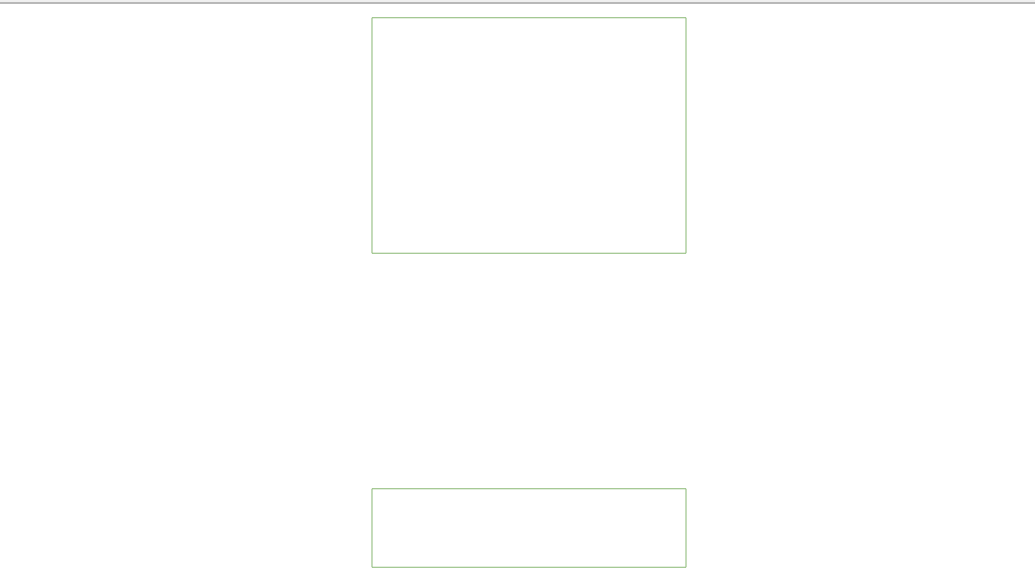
\includegraphics[width=12cm]{figures/1174039/gambar/hasil9.PNG}
		\centering
		\caption{Polygon}
	\end{figure}
	
	\item 
	\lstinputlisting{src/1/1174039/soal10.py}
	\begin{figure}[H]
		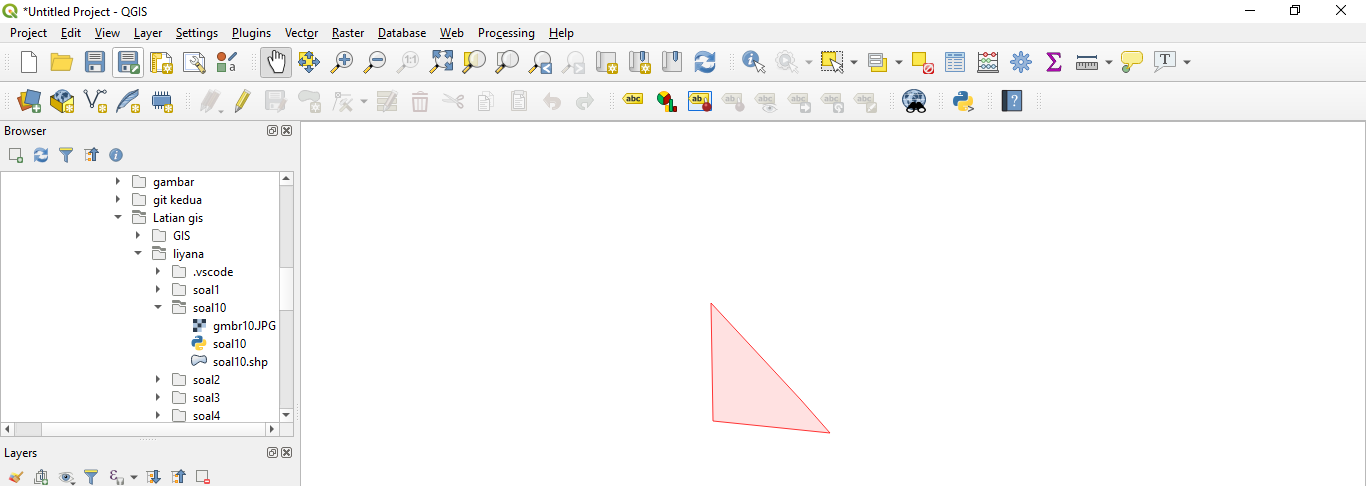
\includegraphics[width=12cm]{figures/1174039/gambar/hasil10.PNG}
		\centering
		\caption{Hasil mod saya yaitu 7 jadi yang saya kerjakan segitiga siku-siku , Polygon}
	\end{figure}	
\end{enumerate}

\subsection{Link}
\href{https://youtu.be/tM_PguRyR4A}{Youtube}
\section{Irvan Rizkiansyah(1174043)}
	\subsection{PySHP}
		\begin{enumerate}
			\item 
				\lstinputlisting{src/1/1174043/nomor1.py}
				\begin{figure}[H]
					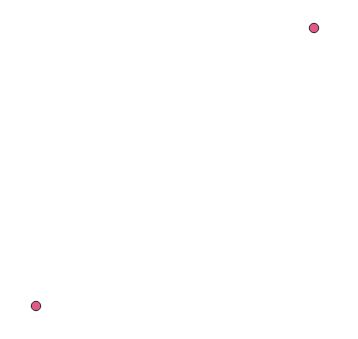
\includegraphics[width=12cm]{figures/1174043/1.jpg}
					\centering
					\caption{Nomor1}
				\end{figure}
			
			\item 
				\lstinputlisting{src/1/1174043/nomor2.py}
				\begin{figure}[H]
					
\includegraphics[width=12cm]{figures/1174043/2.jpg}
					\centering
					\caption{Nomor2}
				\end{figure}
			
			\item 
				\lstinputlisting{src/1/1174043/nomor3.py}
				\begin{figure}[H]
					
\includegraphics[width=12cm]{figures/1174043/3.jpg}
					\centering
					\caption{Nomor3}
				\end{figure}
			
			\item 
				\lstinputlisting{src/1/1174043/nomor4.py}
				\begin{figure}[H]
					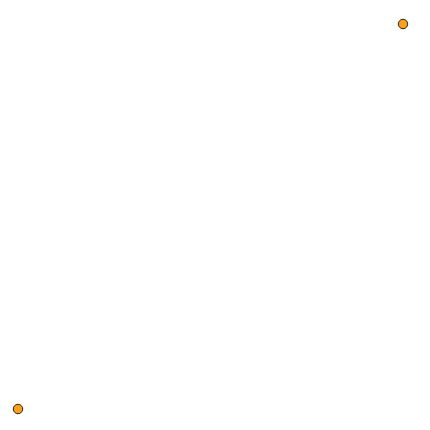
\includegraphics[width=12cm]{figures/1174043/4.jpg}
					\centering
					\caption{Nomor4}
				\end{figure}
			
			\item 
				\lstinputlisting{src/1/1174043/nomor5.py}
				\begin{figure}[H]
					
\includegraphics[width=12cm]{figures/1174043/5.jpg}
					\centering
					\caption{Nomor5}
				\end{figure}
			
			\item 
				\lstinputlisting{src/1/1174043/nomor6.py}
				\begin{figure}[H]
					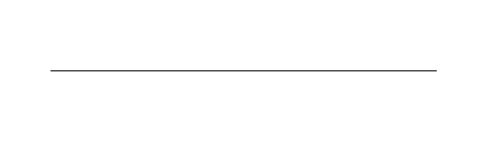
\includegraphics[width=12cm]{figures/1174043/6.jpg}
					\centering
					\caption{Nomor6}
				\end{figure}
			
			\item 
				\lstinputlisting{src/1/1174043/nomor7.py}
				\begin{figure}[H]
					
\includegraphics[width=12cm]{figures/1174043/7.jpg}
					\centering
					\caption{Nomor7}
				\end{figure}
			
			\item 
				\lstinputlisting{src/1/1174043/nomor8.py}
				\begin{figure}[H]
					
\includegraphics[width=12cm]{figures/1174043/8.jpg}
					\centering
					\caption{Nomor8}
				\end{figure}
			
			\item 
				\lstinputlisting{src/1/1174043/nomor9.py}
				\begin{figure}[H]
					
\includegraphics[width=12cm]{figures/1174043/9.jpg}
					\centering
					\caption{Nomor9}
				\end{figure}
			
			\item 1174043 mod 8 = 3, maka bentuk persegi banjang sebanyak 3 buah.
				\lstinputlisting{src/1/1174043/nomor10.py}
				\begin{figure}[H]
					
\includegraphics[width=12cm]{figures/1174043/10.jpg}
					\centering
					\caption{Nomor10}
				\end{figure}	
		\end{enumerate}
		
	\subsection{Link video PySHP - QGIS}
		\href{https://youtu.be/ojRLi8rJ4B8} {Link video PySHP - QGIS Irvan Rizkiansyah - 1174043}


%\chapter{Tugas Kedua}
%\section{NAMA (NPM)}
\subsection{Pengertian}
\subsection{Sejarah}
\subsection{Koordinat}
\subsection{Data Geospasial}
\subsection{Link}
\subsection{Plagiarism}

\subsection{Cara Penggunaan}
\subsubsection{Gambar}

\hfill\break

Contoh Gambar
\begin{figure}[H]
	
\includegraphics[width=4cm]{figures/himatif.png}
	\centering
	\caption{Contoh gambar.}
\end{figure}

\subsubsection{List}
\begin{enumerate}
	\item Satu
	\item Dua
\end{enumerate}

\begin{itemize}
	\item Satu
	\item Dua
\end{itemize}


\bibliographystyle{IEEEtran}
%\def\bibfont{\normalsize}
\bibliography{references}
%%%%%%%%%%%%%%%%%%%%%%%%%%%%%%%%%%%%%%%%%%%%%%


%%%%%%%%%%%%%%%
%%  The default LaTeX Index
%%  Don't need to add any commands before \begin{document}
\printindex

%%%% Making an index
%%
%% 1. Make index entries, don't leave any spaces so that they
%% will be sorted correctly.
%%
%% \index{term}
%% \index{term!subterm}
%% \index{term!subterm!subsubterm}
%%
%% 2. Run LaTeX several times to produce <filename>.idx
%%
%% 3. On command line, type  makeindx <filename> which
%% will produce <filename>.ind
%%
%% 4. Type \printindex to make the index appear in your book.
%%
%% 5. If you would like to edit <filename>.ind
%% you may do so. See docs.pdf for more information.
%%
%%%%%%%%%%%%%%%%%%%%%%%%%%%%%%

%%%%%%%%%%%%%% Making Multiple Indices %%%%%%%%%%%%%%%%
%% 1.
%% \usepackage{multind}
%% \makeindex{book}
%% \makeindex{authors}
%% \begin{document}
%%
%% 2.
%% % add index terms to your book, ie,
%% \index{book}{A term to go to the topic index}
%% \index{authors}{Put this author in the author index}
%%
%% \index{book}{Cows}
%% \index{book}{Cows!Jersey}
%% \index{book}{Cows!Jersey!Brown}
%%
%% \index{author}{Douglas Adams}
%% \index{author}{Boethius}
%% \index{author}{Mark Twain}
%%
%% 3. On command line type
%% makeindex topic
%% makeindex authors
%%
%% 4.
%% this is a Wiley command to make the indices print:
%% \multiprintindex{book}{Topic index}
%% \multiprintindex{authors}{Author index}

\end{document}

